\chapter{The O'Briens in Boston}

The O'Briens\index{O'Brien!family} were among the almost 1.5 million Irish who sailed to the United States between 1845 and 1855.\cite{Miller:291} William\textsuperscript{1}'s\index{O'Brien!William\textsuperscript{1}} two youngest children, Michael\textsuperscript{2}\index{O'Brien!Michael\textsuperscript{2}} and Mary\textsuperscript{2},\index{O'Brien!Mary\textsuperscript{2} (Ward)}\index{Ward, Mary\textsuperscript{2}} were likely the first of the O'Brien family\index{O'Brien!family} to make the voyage. Irish families often could only afford tickets for one or two people, and so would choose the youngest and healthiest children.\cite{Miller:292} Once in America, the children would send remittances back to Ireland\index{Ireland} until the rest of the family could be brought over.\cite{Miller:295}

\begin{figure}
	\centering
	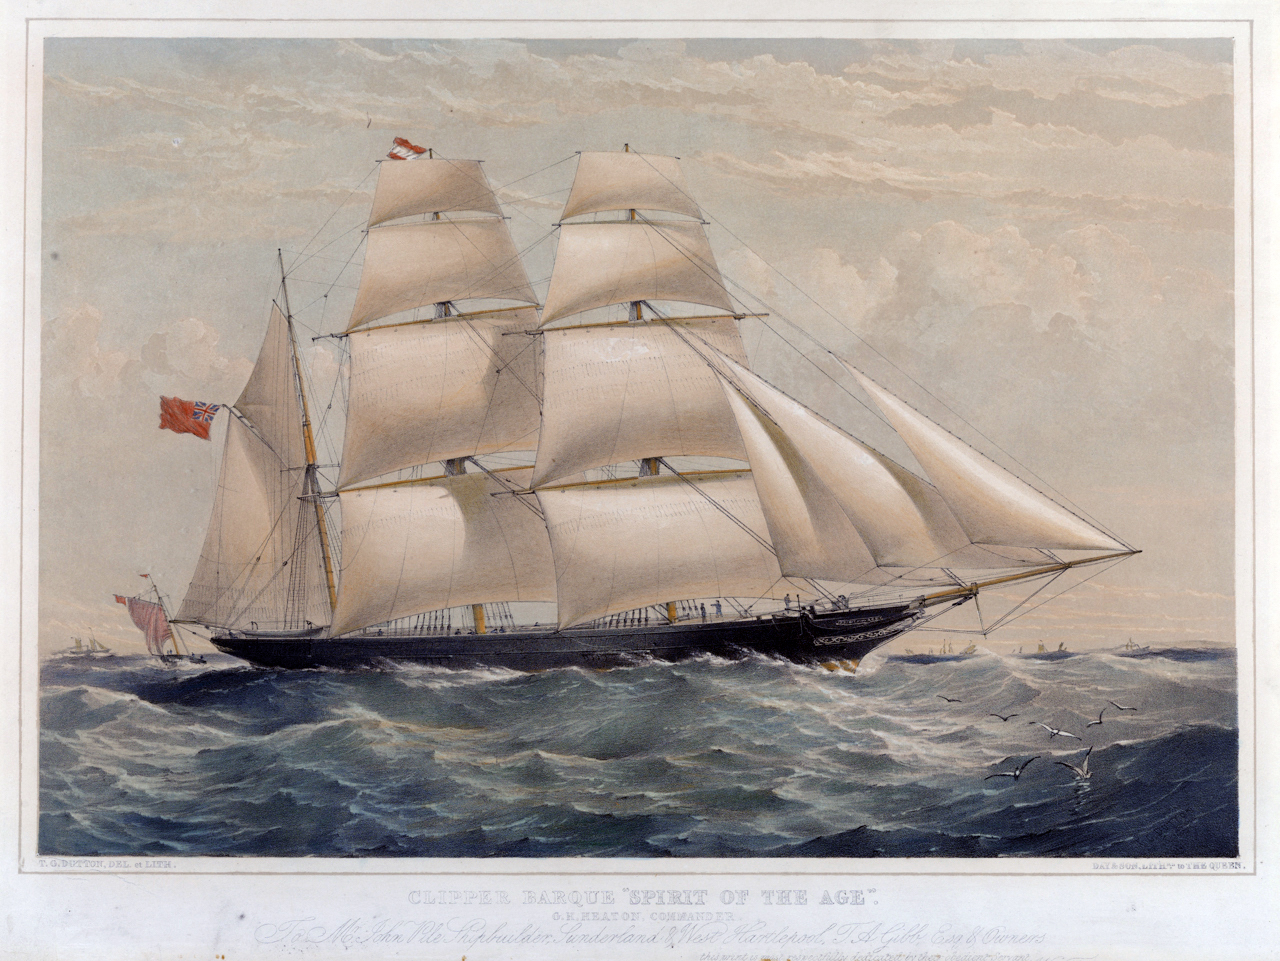
\includegraphics[width=\textwidth]{clipper_barque}
	\caption{Example of a clipper barque\index{clipper barque/bark} from 1854. Thomas Goldsworthy Dutton, ``Clipper barque Spirit of the Age,'' Royal Museums Greenwich (\url{https://commons.wikimedia.org/wiki/File:Clipper_barque_Spirit_of_the_Age,_PY0633.jpg}).}
\end{figure}

\begin{figure}
	\centering
	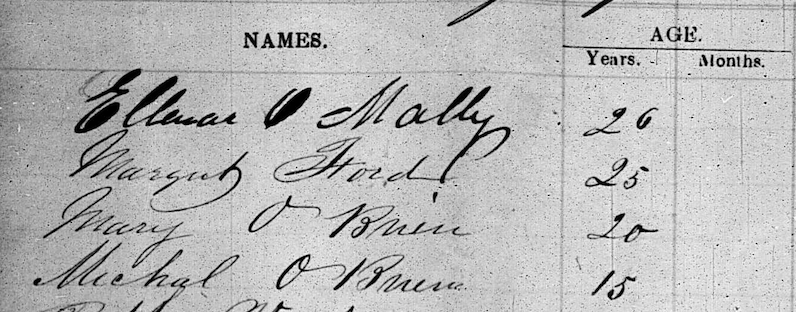
\includegraphics[width=\textwidth]{mary_michael}
	\caption{Passenger list of the \textit{Thomas Baker}\index{Thomas Baker (ship)} showing Mary O'Brien\index{O'Brien!Mary\textsuperscript{2}}\index{Ward, Mary\textsuperscript{2} (Ward)} and Michael O'Brien.\index{O'Brien!Michael\textsuperscript{2}}\cite{ThomasBaker}}
\end{figure}

\begin{figure}
	\centering
	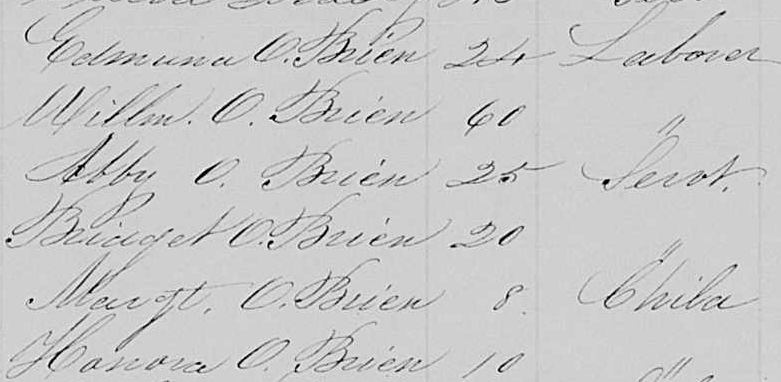
\includegraphics[width=\textwidth]{edward_ship}
	\caption{Passenger list of the \textit{Chasca}\index{Chasca (ship)} showing O'Brien family along with ages and occupations.\cite{Chascay}}
\end{figure}

Ship passenger lists for the Port of New York\index{New York City} show a Mary O'Brien,\index{O'Brien!Mary\textsuperscript{2}}\index{Ward!Mary\textsuperscript{2} (O'Brien)} age 20, and Michael O'Brien,\index{O'Brien!Michael\textsuperscript{2}} age 15, arriving on the brig \textit{Thomas Baker}\index{Thomas Baker (ship)} from Galway, Ireland,\index{Ireland!Galway, County Galway} on 3 July 1849. There were 93 total passengers aboard. The occupation listed for everyone on the passenger manifest is ``farming.''\index{Farming}\cite{ThomasBaker}

Brigs\index{Brigs} like the \textit{Thomas Baker}\index{Thomas Baker (ship)} were two-masted ships with square sails.\cite{OHanlon:35} Prior to the famine,\index{Famine} these ships were outfitted for cargo rather than passengers.\cite{Laxton:9} The \textit{Thomas Baker},\index{Thomas Baker (ship)} for instance, was a coal-hauling ship.\cite{MorningAdvertiser} Compared to the three-masted liners, brigs\index{Brigs} were cramped for the number of passengers they carried, with poor ventilation and five-foot ceilings.\cite{OHanlon:33} The voyage from Ireland\index{Ireland} to the United States took anywhere from four to eight weeks.

A larger group of the O'Briens\index{O'Brien!family} arrived in Boston on 27 June 1851 on board the vessel \textit{Chasca}\cite{Chascay}.\index{Chasca (ship)} The voyage from Liverpool, England,\index{England!Liverpool} to Boston, Massachusetts,\index{Massachusetts!Boston} took 47 days.\cite{Chascay2} On board were Edward\textsuperscript{2} O'Brien\index{O'Brien!Edward/Edmund\textsuperscript{2}} (appearing as Edmund\cite{Edmund}), his father William,\index{O'Brien!William\textsuperscript{1}} wife Bridget\index{Linnehan!Bridget}\index{O'Brien!Bridget (Linnehan)}, sister Abby\textsuperscript{2} (O'Brien) Dooley,\index{O'Brien!Abigail\textsuperscript{2}}\index{Dooley!Abigail\textsuperscript{2} (O'Brien)} and Abby's two children, Margaret\textsuperscript{3}\index{Dooley!Margaret\textsuperscript{3}}\index{Fernald!Margaret\textsuperscript{3} (Dooley)}\index{Simonds!Margaret\textsuperscript{3} (Dooley) (Fernald)} and Hanora\textsuperscript{3} (aka Hannah).\index{Dooley!Hannah/Hanora\textsuperscript{3}}\index{Cooney!Hannah/Hanora\textsuperscript{3} (Dooley)}\index{Cusick!Hannah/Hanora\textsuperscript{3} (Dooley) (Cooney)} There were a total of 256 passengers on board,\cite{Chascay3} which must have made the ship quite crowded. The \textit{Chasca}\index{Chasca (ship)} was a 658-ton clipper bark\index{clipper barque/bark} built in East Boston\index{Massachusetts!Boston!East Boston} as a speedy cargo ship\cite{ChascaCard,Chascay} Like the \textit{Thomas Baker}\index{Thomas Baker (ship)}, it was probably retrofitted to carry passengers in response to the large demand for transport to the New World during the famine\index{famine} years.

Both Abby's\index{Dooley!Abigail\textsuperscript{2} (O'Brien)}\index{O'Brien!Abigail\textsuperscript{2}} and Margaret's\index{Dooley!Margaret\textsuperscript{3}}\index{Fernald!Margaret\textsuperscript{3} (Dooley)}\index{Simonds!Margaret\textsuperscript{3} (Dooley) (Fernald)} occupations are listed as ``Servt.''\index{servant} in the passenger manifest.\cite{Chascay} About 2,000 Irish women\index{Irish-Americans} in Boston\index{Massachusetts!Boston} were domestic workers\index{Domestic workers} in 1850. It was a popular trade for Irish\index{Irish-Americans} immigrant women since they spoke English and didn't have many other opportunities for work available to them.\cite{Ryan:41}

William's\index{O'Brien!William\textsuperscript{1}} remaining two children, John\textsuperscript{2}\index{O'Brien!John\textsuperscript{2}} and Ann\textsuperscript{2},\index{O'Brien!Ann\textsuperscript{2}}\index{Dailey!Ann\textsuperscript{2} (O'Brien)} made separate voyages from Ireland\index{Ireland} to Boston\index{Massachusetts!Boston} but cannot be found in passenger records. John\index{O'Brien!John\textsuperscript{2}} must have arrived sometime prior to his marriage in 1853.\cite{John2OBrienCivilMarriage} Ann\index{O'Brien, Ann\textsuperscript{2}}\index{Daily, Ann\textsuperscript{2} (O'Brien)} may not have arrived until 1870--1880 as she doesn't appear in any prior records.\cite{Census1880Edward} 

Like other Irish\index{Irish-Americans} immigrants from this time period, William O'Brien\index{O'Brien!William\textsuperscript{1}} and his children likely came to America to escape the famine\index{famine} and build a better life. While the family may have avoided starvation in Ireland,\index{Ireland} the first few years in Boston\index{Massachusetts!Boston} presented new challenges. The O'Briens\index{O'Brien!family} lived in crowded tenement buildings, suffered devastating losses from communicable diseases, and likely faced anti-Catholic\index{Catholicism} discrimination from the city's dominant class of Protestants.\index{Protestantism}\cite{Ryan:61,Quinlan:58}
	
Moving frequently at first, the family lived predominantly in Boston's North End\index{Massachusetts!Boston!North End} neighborhood during the 1850s and 1860s.\cite{NorthEndAddresses} In 1855, half of all residents of the North End\index{Massachusetts!Boston!North End} were Irish.\index{Irish-Americans}\cite{Todisco:29} Landlords had subdivided the North End's old mansions and warehouses into crowded tenement houses for renting to the newly-arrived immigrants.\cite{Goldfeld:102} Many of the tenements were not connected to sewage systems or had defective toilets, leading to high rates of infant mortality and diseases like smallpox, cholera, and tuberculosis.\cite{Goldfeld:103,Todisco:21,Ryan:48}

In 1834, Irish immigrants\index{Irish-Americans} founded the first Catholic church\index{Catholicism} in Boston's North End\index{Massachusetts!Boston!North End} --- St.\ Mary's of the Sacred Heart,\index{St.\ Mary's of the Sacred Heart (church)} on the corner of Endicott\index{Massachusetts!Boston!Endicott St.} and Cooper Streets.\index{Massachusetts!Boston!Cooper St.}\cite{Todisco:26} John O'Brien\index{O'Brien!John\textsuperscript{2}} married Mary Mahony\index{Mahoney!Mary}\index{O'Brien!Mary (Mahoney)}\index{Bowser, Mary (Mahoney) (O'Brien)} there in 1853.\cite{John2OBrienMarriage} St.\ Mary's\index{St.\ Mary's of the Sacred Heart (church)} quickly reached capacity, and so in 1843, St.\ John the Baptist Church\index{St.\ John the Baptist (church)} was founded in a converted pork storehouse on Moon St.\index{Massachusetts!Boston!Moon St.}\cite{Goldfeld:101,Sullivan:128} John's children Mary\textsuperscript{3}\index{O'Brien!Mary\textsuperscript{3} (1856--1883)} and Ellen\textsuperscript{3}\index{O'Brien, Ellen\textsuperscript{3} (1859--1882)} were baptized there. St.\ John's,\index{St. John the Baptist (church)} too, became crowded, which in 1862 lead to the Catholics\index{Catholicism} purchasing the New North Church\index{New North Church} at the corner of Hanover\index{Massachusetts!Boston!Hanover St.} and Clark Streets\index{Massachusetts!Boston!Clark St.} and re-dedicating it as St.\ Stephen's.\index{St. Stephen's (church)}\cite{Sullivan:128} The O'Brien family\index{O'Brien!family} followed many other Irish\index{Irish-Americans} in moving from St.\ John's\index{St. John the Baptist (church)} to St.\ Stephen's\index{St. Stephen's (church)} when it opened. The O'Briens' baptisms and marriages took place at St.\ Stephen's\index{St. Stephen's (church)} at least until Margaret Dooley's\index{Dooley!Margaret\textsuperscript{3}}\index{Fernald!Margaret\textsuperscript{3} (Dooley)}\index{Simonds!Margaret\textsuperscript{3} (Dooley) (Fernald)} marriage there in 1873.\cite{RobertFernaldMarriage}

\begin{figure}
	\centering
	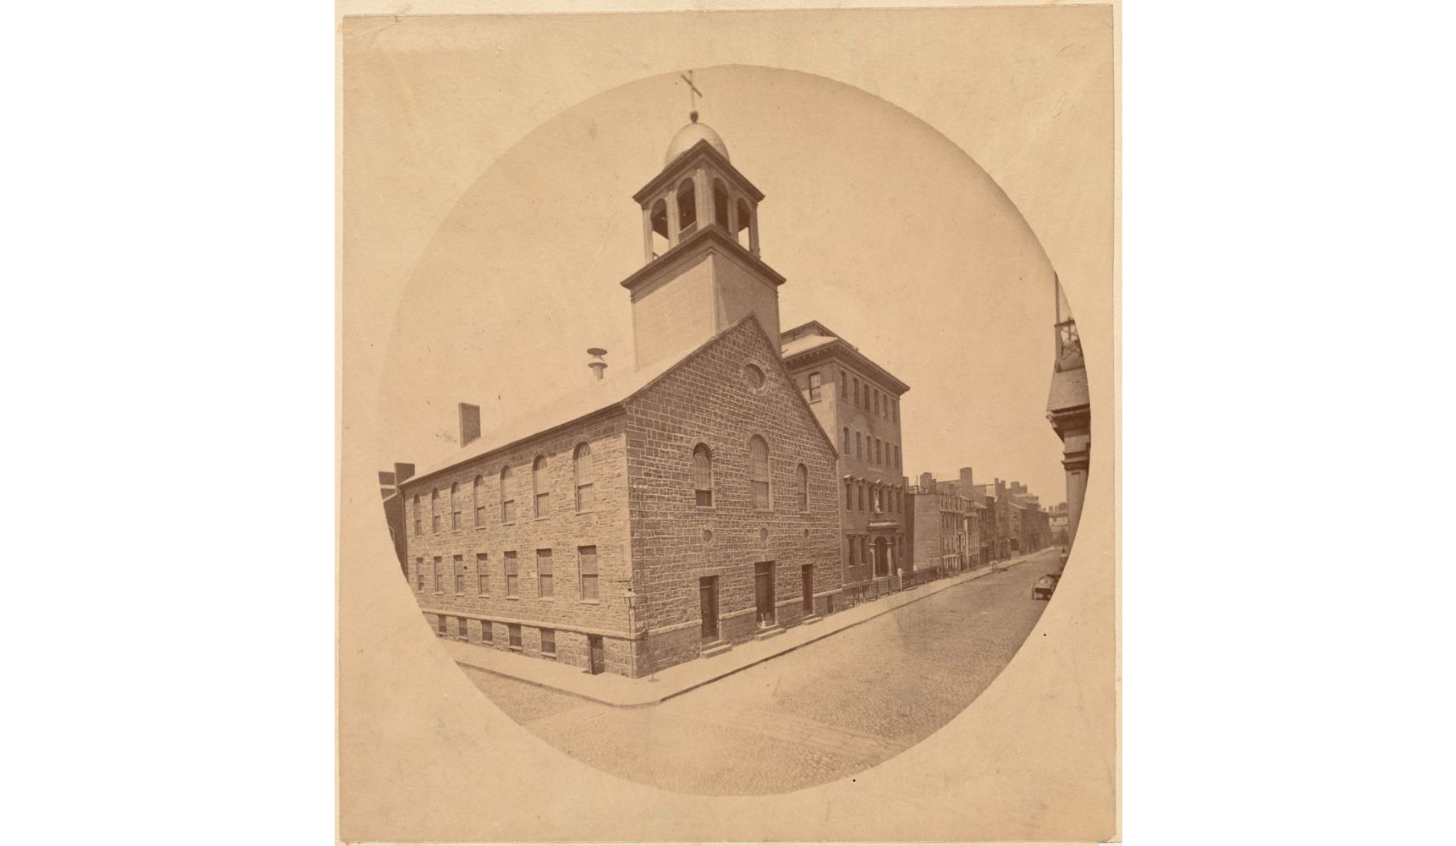
\includegraphics[width=\textwidth]{st_marys}
	\caption{Josiah Johnson Hawes, ``Old St.\ Mary's Church, Endicott ad Cooper Sts.,''\index{St.\ Mary's of the Sacred Heart (church)} photograph, 1860, Boston Public Library Arts Department (\url{https://ark.digitalcommonwealth.org/ark:/50959/c821h611m}).}
\end{figure}

Irish\index{Irish-Americans} immigrants to Boston\index{Massachusetts!Boston} had difficulty finding steady work, given that they were mostly rural farmers\index{farming} and did not have specialized trade skills.\cite{Ryan:21} Many of them started out by opening a grocery\index{grocery} store in their tenement house or somewhere close by.\cite{Ryan:83} Indeed, John's\index{O'Brien!John\textsuperscript{2}} occupation is listed as ``grocer''\index{grocery} on his son John Joseph's\index{O'Brien!John Joseph\textsuperscript{3} (1861--1938)} birth record.\cite{John3OBrienBirth} 

John\index{O'Brien!John\textsuperscript{2}} and his brother Michael\index{O'Brien!Michael\textsuperscript{2}} both worked as oystemen.\index{oyster harvesting}\cite{EdwardFrancis3OBrienBirth,Michael2OBrien1886,1861John2OBrien} Before the advent of industrial-scale dredging operations, the traditional method of oyster harvesting\index{oyster harvesting} used tongs. Oyster tongs consisted of a pair of metal rakes at the end of long wooden shafts. The oysterman\index{oyster harvesting} would use the tongs to scrape oysters off the bottom of the sea bed and manually haul them onto the boat, up to 70 pounds at a time. The boats were small vessels rigged with one or two sails.\cite{Botwick:95} Being an oysterman\index{oyster harvesting} brought a degree of independence for an unskilled laborer. He typically owned his own boat and tackle, shucked the oysters at home to sell locally, and kept all the profits.\cite{MacKenzie:7, Botwick:96} This changed beginning in the 1870s when steam-powered oyster dredging ships arrived, and packing houses took over the oyster shucking process.\cite{MacKenzie:5, MacKenzie:7} The O'Brien brothers may have sailed to Wellfleet Harbor, Massachusetts,\index{Massachusetts!Wellfleet} which had plentiful oyster beds seeded with oysters from New Haven, Connecticut.\cite{MacKenzie:29}

\begin{figure}
	\centering
	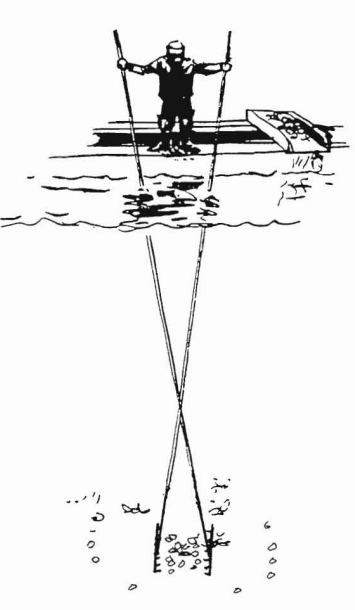
\includegraphics[width=0.3\textwidth]{oyster_tongs}
	\caption{Use of oyster tongs.\index{oyster harvesting}\cite{MacKenzie:4}}
\end{figure}

\begin{figure}
	\centering
	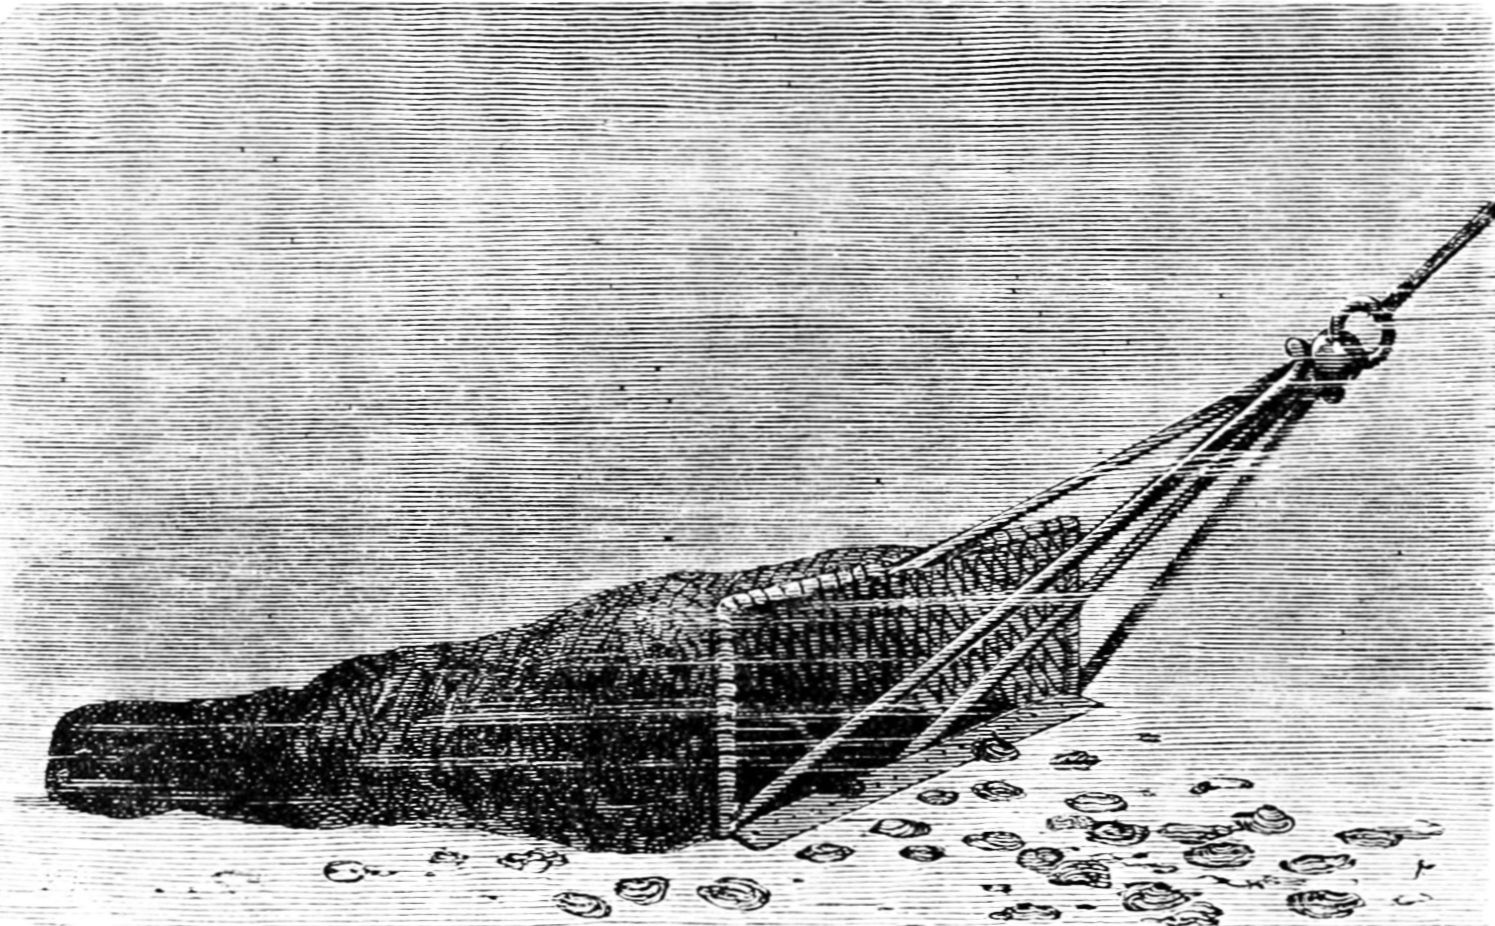
\includegraphics[width=0.8\textwidth]{oyster_dredge}
	\caption{An oyster dredge at work,\index{oyster harvesting} c.\ 1875, Popular Science Monthly Volume 6 (\url{https://commons.wikimedia.org/wiki/File:PSM_V06_D020_An_oyster_dredge_at_work.jpg}).}
\end{figure}

It seems that Edward\index{O'Brien!Edward/Edmund\textsuperscript{2}} was the main provider for the O'Brien family\index{O'Brien!family} during the early years in Boston.\index{Massachusetts!Boston} He may have had a successful trade in Ireland\index{Ireland} prior to his arrival in the United States. In 1855 he was housing his father and his sister Abby's\index{Dooley!Abigail\textsuperscript{2} (O'Brien)}\index{O'Brien!Abigail\textsuperscript{2}} family in addition to his own.\cite{Census1855William} Edward\index{O'Brien!Edward/Edmund\textsuperscript{2}} purchased a 2-person cemetery plot at North Cambridge Catholic Cemetery\index{North Cambridge Catholic Cemetery} in 1852\cite{CarolGordon} and a large 13-person plot at Holy Cross Cemetery\index{Holy Cross Cemetery} in 1880\cite{HolyCrossPlot} where many of his family members were buried.

In the early 1870s, most of William's\index{O'Brien!William\textsuperscript{1}} adult children (Edward,\index{O'Brien!Edward/Edmund\textsuperscript{2}} Ann,\index{O'Brien!Ann\textsuperscript{2}}\index{Daily!Ann\textsuperscript{2} (O'Brien)} Mary,\index{O'Brien!Mary\textsuperscript{2}}\index{Ward!Mary\textsuperscript{2} (O'Brien)} and Michael\index{O'Brien!Michael\textsuperscript{2}}) relocated to East Boston.\index{Massachusetts!Boston!East Boston} John's\index{O'Brien!John\textsuperscript{2}} sons, John Joseph\textsuperscript{3},\index{O'Brien!John Joseph\textsuperscript{3} (1861--1938)} James Edward\textsuperscript{3},\index{O'Brien!James Edward\textsuperscript{3}} and William\textsuperscript{3},\index{O'Brien!William\textsuperscript{3}} moved to Boston's South Cove\index{Massachusetts!Boston!South Cove} neighborhood (now part of Chinatown\index{Massachusetts!Boston!Chinatown}).\cite{1870sAddresses}

John's\index{O'Brien!John\textsuperscript{2}} family was hit particularly hard by tuberculosis.\index{tuberculosis}\index{phthisis|see {tuberculosis}}\index{consumption|see {tuberculosis}}\footnote{The terms ``phthisis'' and ``consumption'' were used at the time to describe what is now called tuberculosis.\cite{TuberculosisHistory}} Four of his children died of the disease between 1879 and 1889, as did John\index{O'Brien!John\textsuperscript{2}} himself in 1863.\cite{John2OBrienDeath} In fact, John's line would have ended if not for his son John Joseph.\index{O'Brien!John Joseph\textsuperscript{3} (1861--1938)} Tuberculosis\index{tuberculosis} disproportionately affected Irish immigrants\index{Irish-Americans} in Boston:\index{Massachusetts!Boston}

\begin{quote}
	...[t]he death rate from consumption\index{tuberculosis} was greatest among the colored, and among the white ... it was greatest among those whose mothers were born in Ireland\index{Ireland}\index{Irish-Americans} or who were themselves natives of Ireland, being more than 3 times the corresponding rate for those whose mothers were born in the United States, and almost double the rate for those who were themselves natives of this country.\cite{VitalStatistics}
\end{quote}

Three of Michael's\index{O'Brien!Michael\textsuperscript{2}} sons had jobs working in Boston's\index{Massachusetts!Boston} gas industry.\index{gas industry} Their roles included gas meter maker, meter tester, meter reader, and foreman. The Boston Gas Company\index{Boston Gas Company} constructed a large coal gas plant at Commercial Point\index{Massachusetts!Boston!Commercial Point} in 1882. The company needed to hire a large number of unskilled laborers, and many of them were Irish\index{Irish-Americans} immigrants.\cite{Keating:11} In the early 20th century, these jobs were highly valued, as the company (later called Boston Consolidated Gas)\index{Boston Consolidated Gas} offered employee profit-sharing plans in 1906 and a pension plan in 1919. This provided job stability and wealth for the Irish\index{Irish-Americans} working class.\cite{Keating:20}

The profiles later in this report include details about each descendant of William O'Brien\index{O'Brien!William\textsuperscript{1}} through the 4th generation.
